\section{Experiments}
\label{sec:experiments}

In this section, we evaluate the system performance of the proposed MXFP4 training framework, focusing on training throughput, memory footprint, and recomputation efficiency.

\subsection{Experimental setup}
\textbf{Hardware \& Environment}. We conduct all experiments on a cluster of 32 nodes, equipped with a total of 256 NVIDIA Hopper GPUs (80GB HBM3). The GPUs are interconnected via NVSwitch within nodes and InfiniBand across nodes.

\textbf{Model Configuration}. We train a 671B-parameter Mixture-of-Experts (MoE) model featuring the Multi-Head Latent Attention (MLA) architecture. The model configuration follows the public DeepSeek-V3 settings, including the Multi-Head Latent Attention (MLA) architecture, with identical MoE expert and projection-layer dimensions.

\textbf{Baselines}. We compare our system against two strong baselines implemented in Megatron-LM:\\
1. BF16: Standard bfloat16 mixed-precision training.\\
2. FP8: Transformer engine blockwise FP8 recipe  training optimized for Hopper architecture. 

We report the training throughput in Tokens per GPU per Second (TGS) and peak memory usage.
 
\subsection{End-to-End Training Performance}

Table~\ref{tab:main_results} summarizes the performance comparison. Our primary observation is that memory constraints on the 671B model force standard baselines into aggressive recomputation (rematerialization) regimes, limiting their performance. Under the standard setting (checkpointing Attention, LayerNorm, and MoE Experts), our MXFP4 method achieves parity with the FP8 baseline in throughput ($\approx$ 1156 TGS) but reduces memory footprint by 14.8\% . Crucially, this memory headroom allows us to reduce the recomputation scope. When we relax the recomputation strategy to only checkpoint the MLA Up-Projection, both BF16 and FP8 baselines encounter Out-of-Memory (OOM) errors. In contrast, our system operates efficiently within the memory limit (70.11\%), achieving a peak throughput of 1302 TGS. This represents a 12.5\% speedup over the best feasible FP8 configuration and a 16.0\% speedup over the BF16 baseline.  

\textbf{Impact of Recomputation Granularity.}
As shown in Table~\ref{tab:main_results}, the 671B model is primarily constrained by the memory wall. Under FP8, fitting the model requires full recomputation of expert layers, introducing substantial redundant computation. By quantizing activations in the MLP and shared MoE expert layers to MXFP4, we reduce peak memory usage by approximately 15\%, which allows us to skip recomputation for these layers. Despite a small quantization overhead, eliminating backward-pass recomputation yields a net throughput gain of 146 TGS (from 1156 to 1302).


\begin{table}[!htbp]
\centering
\resizebox{\linewidth}{!}{
\begin{tabular}{lcccccc}
\toprule
\textbf{Recomputation Scope} & \multicolumn{2}{c}{\textbf{Baseline (BF16)}} & \multicolumn{2}{c}{\textbf{Baseline (FP8)}} & \multicolumn{2}{c}{\textbf{Ours (MXFP4)}} \\
\cmidrule(lr){2-3} \cmidrule(lr){4-5} \cmidrule(lr){6-7}
 & TGS & Mem& TGS & Mem& \textbf{TGS} & \textbf{Mem}\\
\midrule
\textit{Attn + LN + MoE Experts} & 1122 & 68.29\%& 1157 & 74.20\%& 1156 & \textbf{59.40\%}\\
\textit{Attn + LN + MLP} & OOM & - & OOM & - & \textbf{1248} & 60.62\%\\
\textit{MLA Up Proj Only} & OOM & - & OOM & - & \textbf{1302} & 70.11\%\\
\bottomrule
\end{tabular}
}
\caption{Performance on 671B MoE Model.}
\label{tab:main_results}
\end{table}

We conduct additional experiments on a 236B model in table~\ref{tab:236B_main_results} to enable a controlled comparison across numerical precisions under identical recomputation policies, which is not feasible at the 671B scale due to frequent OOM failures of BF16 and FP8. By fixing the recomputation strategy and varying only precision, we show that MXFP4 reduces peak memory usage by 6.9\% compared to blockwise FP8 when FP4 is applied to the MLP and shared experts, and by 7.2\% when FP4 is extended to the entire MoE, corresponding to an 11\% reduction relative to BF16. Under the most aggressive recomputation regime, MXFP4 consistently outperforms FP8 with an average 7.5\% memory reduction, while BF16 still fails to fit into device memory. Together with the 671B results, these findings confirm that applying FP4 to both MLP and MoE components yields substantial and scalable memory benefits.

\begin{table}[!htbp]
\centering
\resizebox{\columnwidth}{!}{
\begin{tabular}{lcccccc}
\toprule
\textbf{Recomputation Scope}
& \multicolumn{2}{c}{\textbf{Baseline (BF16)}}
& \multicolumn{2}{c}{\textbf{Baseline (FP8)}}
& \multicolumn{2}{c}{\textbf{Ours (MXFP4)}} \\
\cmidrule(lr){2-3}
\cmidrule(lr){4-5}
\cmidrule(lr){6-7}
& TGS & Mem
& TGS & Mem
& \textbf{TGS} & \textbf{Mem} \\
\midrule
\textit{Attn + LN + MoE Experts}
& 1725.16 & 53.22\%
& 1621.96 & 56.81\%
& 1608.68 & \textbf{49.96\%} \\
\textit{Attn + LN + MLP}
& 1838.56 & 60.80\%
& 1746.20 & 57.03\%
& 1616.90 & \textbf{49.85\%} \\
\textit{MLP Up Proj Only}
& OOM & -
& 1831.20 & 66.13\%
& 1722.98 & 58.62\% \\
\bottomrule
\end{tabular}
}
\caption{Performance on 236B MoE Model.}
\label{tab:236B_main_results}
\end{table}


% \begin{table}[t]
%   \caption{Comparison of Throughput / Memory Occupation (GB) across precision settings on 671B training. }
%   \label{tab:throughput_memory_compact}
%   \begin{center}
%     \begin{small}
%       \begin{sc}
%         % 调整列间距
%         \setlength{\tabcolsep}{4pt} 
%         \begin{tabular}{lccc}
%           \toprule
%           Recompute Module & BF16 & FP8 & MXFP4 \\
%           & \scriptsize{(TGS / Mem)} & \scriptsize{(TGS / Mem)} & \scriptsize{(TGS / Mem)} \\
%           \midrule
%           Attn. + LN + MoE & 1122 / 68.3 & 1157 / 74.2 & 1156 / 59.4 \\
%           Attn. + LN + MLP & OOM & OOM & 1248 / 60.6 \\
%           MLA Up Proj.     & OOM & OOM & 1302 / 70.1 \\
%           \bottomrule
%         \end{tabular}
%       \end{sc}
%     \end{small}
%   \end{center}
%   \vskip -0.1in
% \end{table}


\subsection{Analysis and Ablation Studies}
To understand the source of our performance gains, we benchmark our custom quantization kernels against the standard Transformer Engine (TE) FP8 baselines. 

\textbf{Fusion Efficiency} 
First, we validate our kernel fusion strategy in Figure~\ref{fig:kernel_fusion}. Evaluated across tensor shapes representative of 236B and 671B training configurations, our approach—which fuses dequantization, data type casting, and layout transformation into a single kernel—achieves a 1.6x–1.9x speedup compared to a naive sequence of separate operations.

\textbf{End-to-End Kernel Performance}
When comparing our total operator latency (Quantization + Fused Dequantization) against the TE FP8 baseline in Figure~\ref{fig:e2e_overhead}, we observe two distinct behaviors:

\begin{itemize}
\item Standard Linear Layers: For standard dense projections (e.g., in Attention blocks), the additional overhead of on-the-fly quantization results in a 0.33x relative speedup (i.e., higher latency) compared to the highly optimized TE baseline.
\item MoE Expert Layers (Group Linear Layers): Crucially, for the computation-heavy MoE expert layers, our specialized msplit kernel significantly outperforms the Transformer Engine FP8 split quantize baseline, achieving a 1.43x–1.53x speedup. This suggests that our custom implementation handles the grouped memory access patterns of MoE experts more efficiently than the generic library calls.
\end{itemize}
Since the MoE expert computation dominates the total FLOPs of the 671B model, this acceleration in the critical path, combined with the reduced recomputation, successfully amortizes the overhead incurred in the standard linear layers, leading to the overall system throughput improvement.

\begin{figure}[htbp]
    \centering
    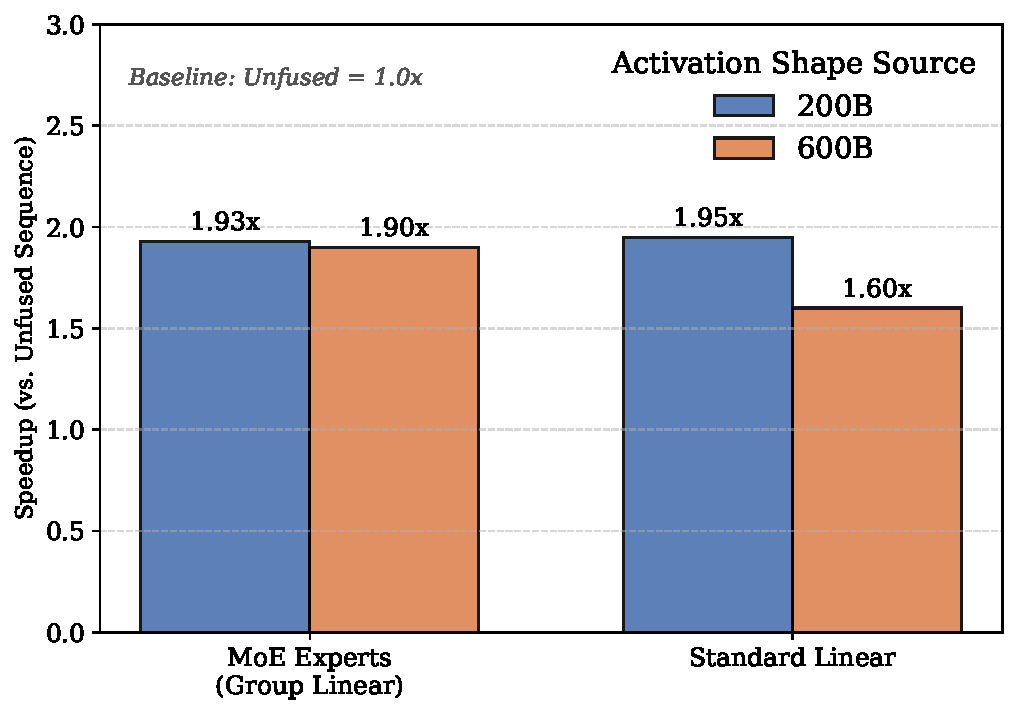
\includegraphics[width=0.9\linewidth]{images/figure_fusion_efficiency_v5.pdf}
    \caption{\textbf{Fusion Efficiency (Fused Kernel vs. Dequant + TE Quant).} 
        Our fused approach achieves consistent speedups (1.6x--1.9x) by eliminating intermediate memory writes.}
    \label{fig:kernel_fusion}
\end{figure}

\begin{figure}[htb]
    \centering
    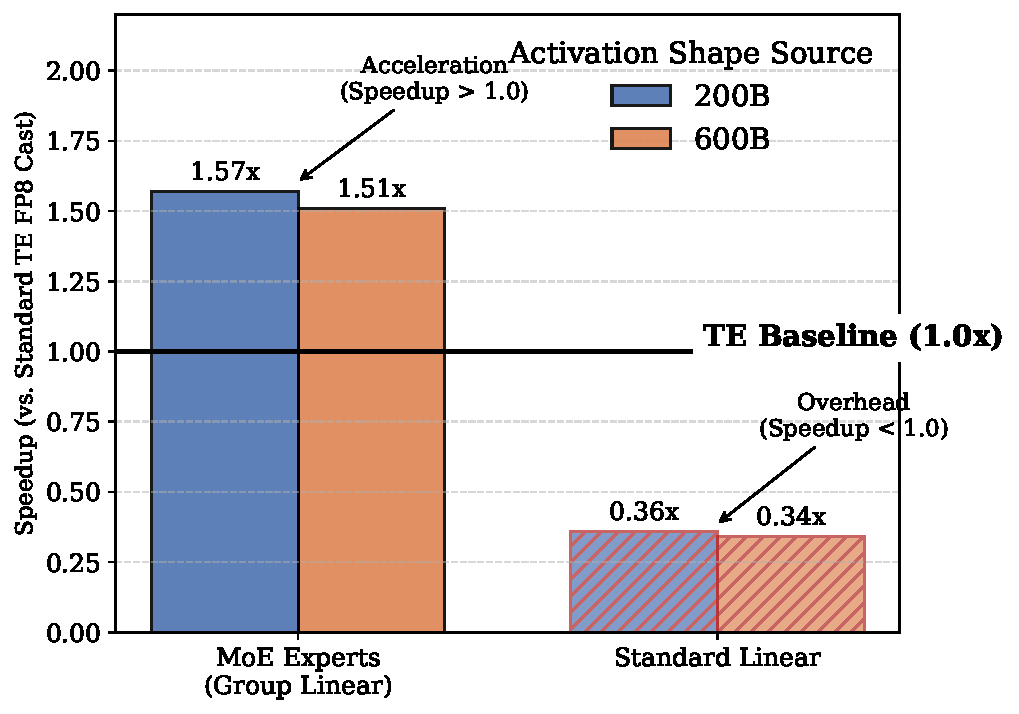
\includegraphics[width=0.9\linewidth]{images/figure_e2e_overhead_v5.pdf}
    \caption{\textbf{Total Quantization Overhead (Ours Full Pipeline vs. TE Baseline).}
        While standard linear layers incur overhead ($<$1.0x), specialized MoE kernels achieve net acceleration ($>$1.5x).}
    \label{fig:e2e_overhead}
\end{figure}


\subsection{Convergence Verification}
To evaluate the training stability of our MXFP4 quantization scheme, we reproduce a configuration consistent with recent large-scale LLM training recipes and the official MXFP4 training methodology. All models are trained using AdamW with a cosine learning rate decay on a 16B-parameter model. We fix the global batch size to 4800 sequences and a context length of 4096 tokens, matching the conditions used in our primary comparisons. The optimizer uses $\beta_1=0.9$, $\beta_2=0.95$, and weight decay of $1.0\times10^{-1}$; gradients are clipped to a global norm of 1.0. We apply the same weight initialization, dropout, and tokenizer settings across BF16 and MXFP4 runs to prevent confounding factors. Both BF16 and MXFP4 experiments are run on identical hardware clusters using the same mixed-precision and tensor-parallel infrastructure.

As illustrated in Figure~\ref{fig:loss}, the loss trajectory of our method strictly follows the BF16 baseline, with no observed instability or divergence. Loss trajectories and quantization-induced deviations are evaluated after consuming 160B training tokens. Quantitatively, FP8 and MXFP4 incur relative loss deviations of $+0.29\%$ and $+0.61\%$ with respect to BF16, respectively, indicating that MXFP4 maintains stable optimization despite more aggressive quantization.

\begin{figure}[htbp]
    \centering
    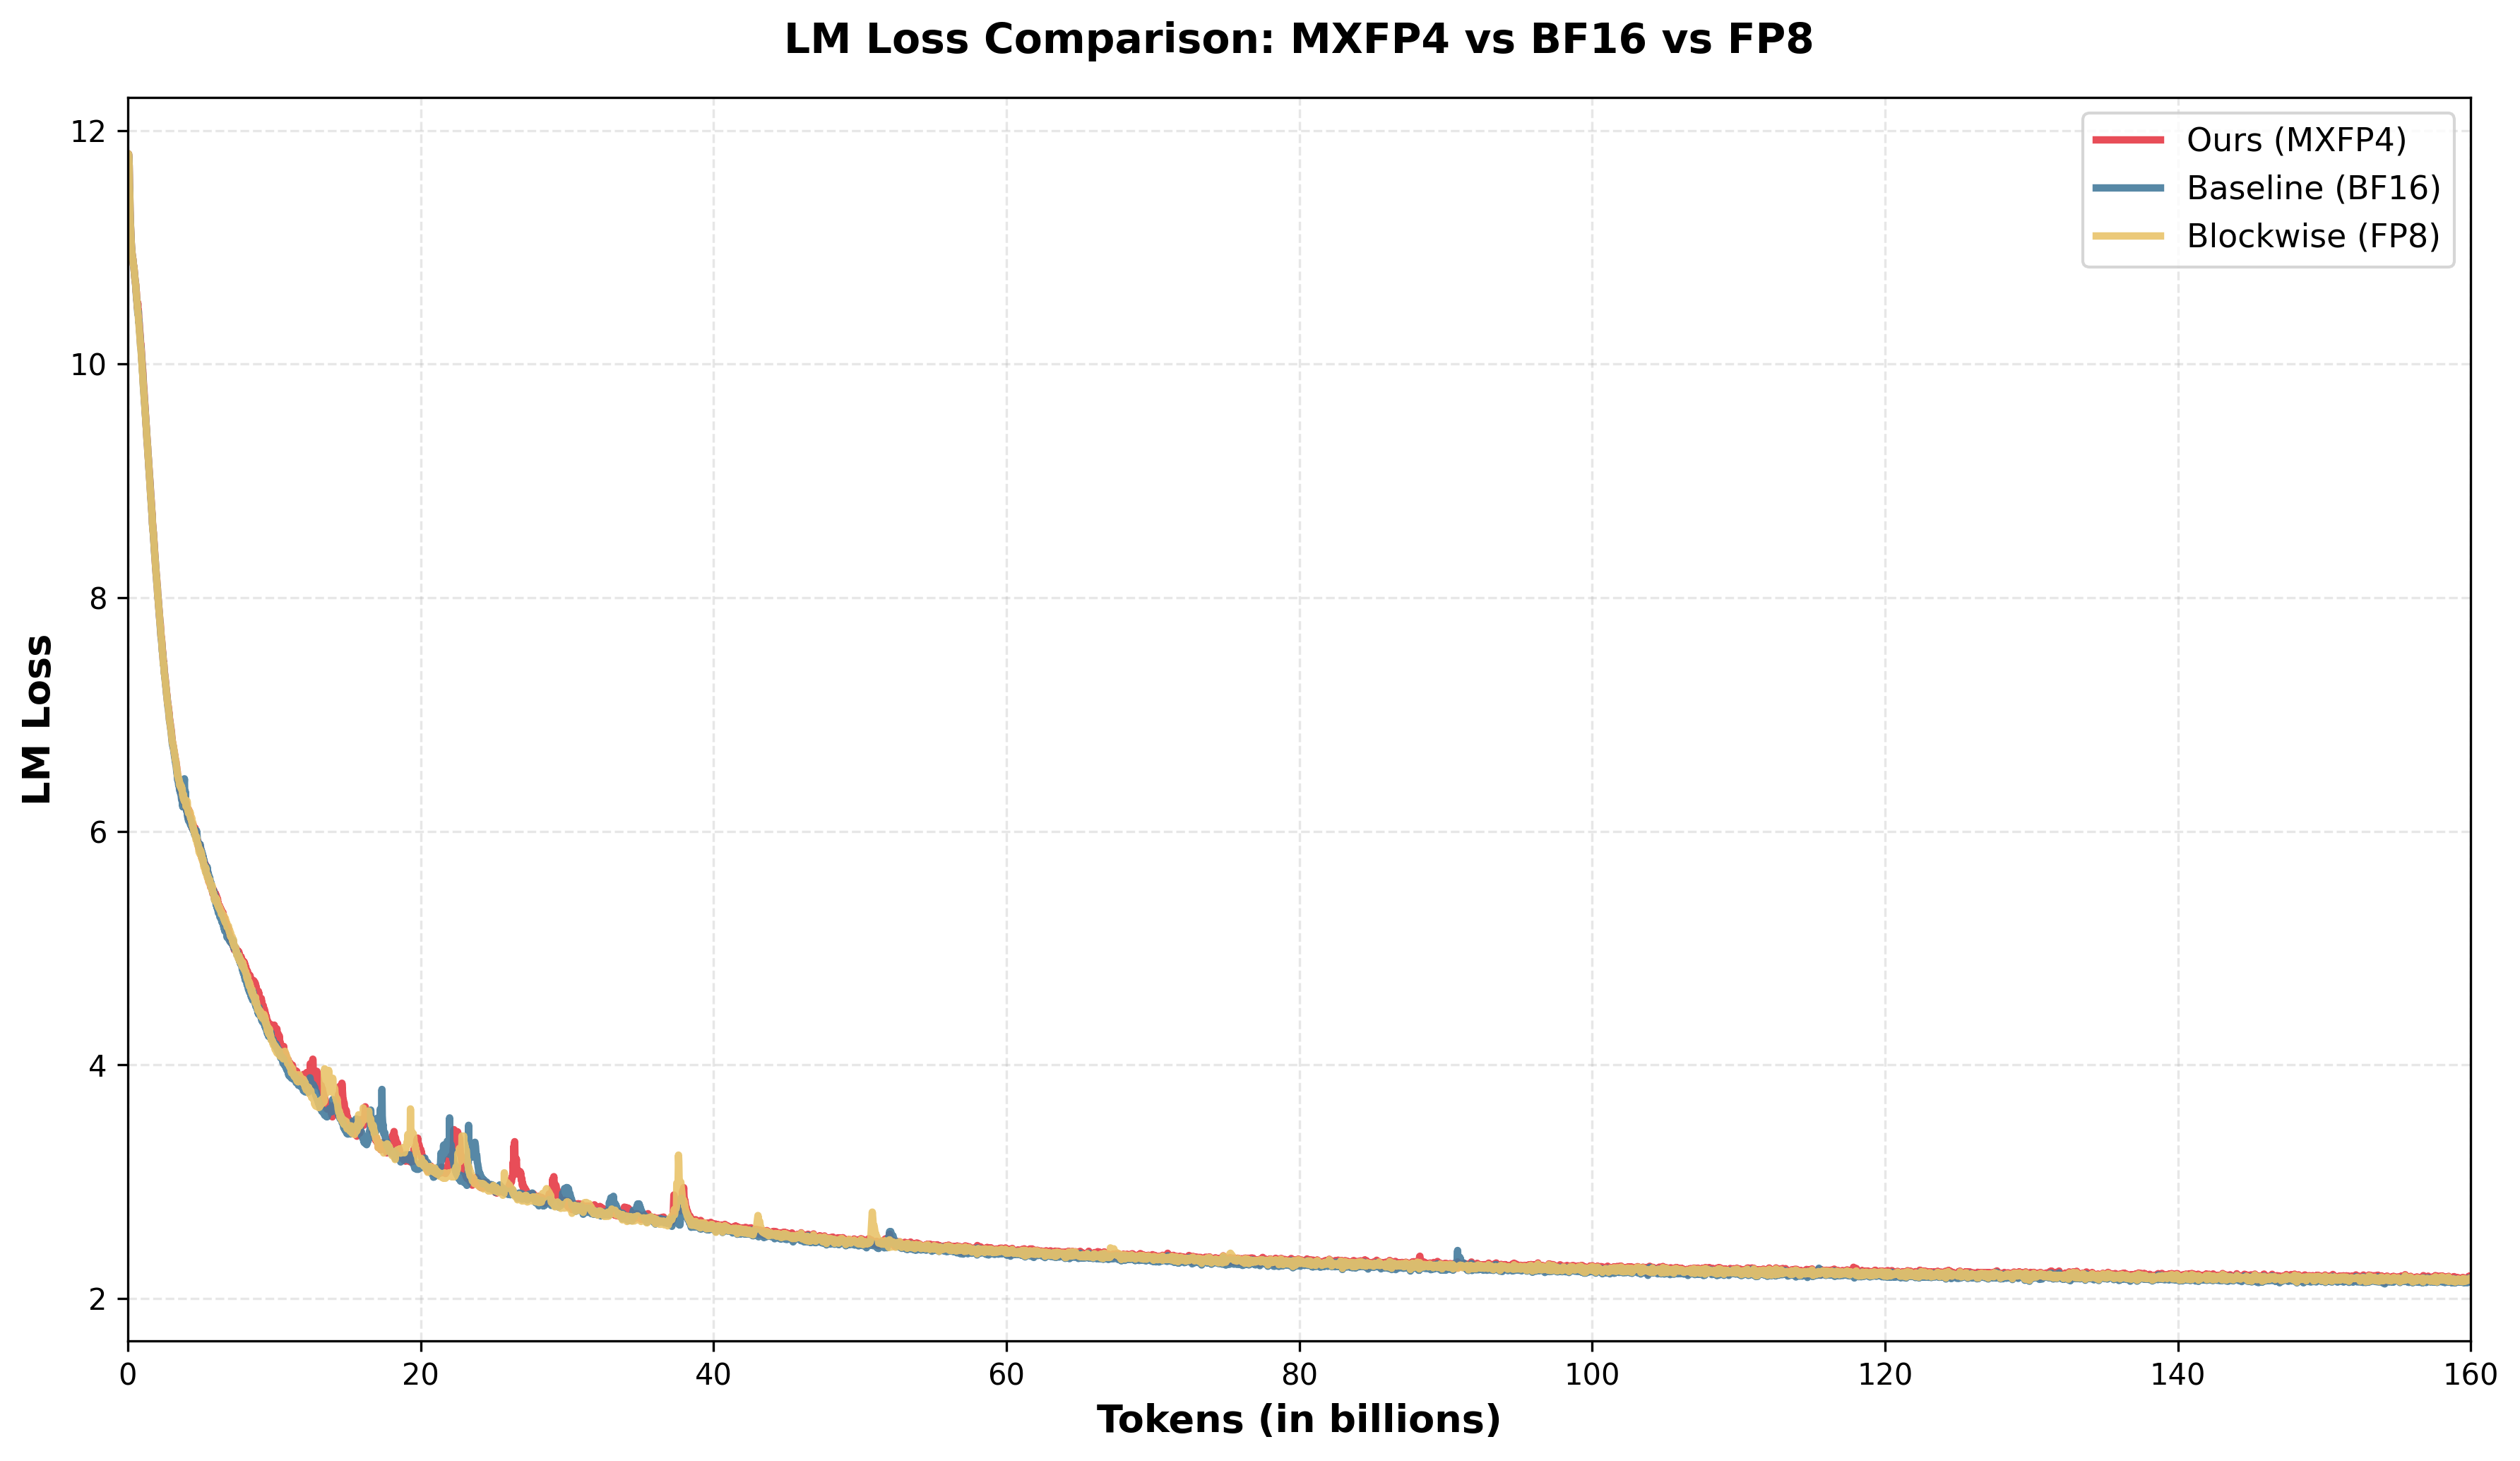
\includegraphics[width=\linewidth]{images/loss.png}
    \caption{LM Loss Comparison.}
    \label{fig:loss}
\end{figure}
